 \chapter{\IfLanguageName{dutch}{Literatuurstudie}{State of the art}}
\label{ch:stand-van-zaken}

% Tip: Begin elk hoofdstuk met een paragraaf inleiding die beschrijft hoe
% dit hoofdstuk past binnen het geheel van de bachelorproef. Geef in het
% bijzonder aan wat de link is met het vorige en volgende hoofdstuk.

% Pas na deze inleidende paragraaf komt de eerste sectiehoofding.
%
%Dit hoofdstuk bevat je literatuurstudie. De inhoud gaat verder op de inleiding, maar zal het onderwerp van de bachelorproef *diepgaand* uitspitten. De bedoeling is dat de lezer na lezing van dit hoofdstuk helemaal op de %hoogte is van de huidige stand van zaken (state-of-the-art) in het onderzoeksdomein. Iemand die niet vertrouwd is met het onderwerp, weet nu voldoende om de rest van het verhaal te kunnen volgen, zonder dat die er nog andere informatie moet over opzoeken \autocite{Pollefliet2011}.

%Je verwijst bij elke bewering die je doet, vakterm die je introduceert, enz. naar je bronnen. In \LaTeX{} kan dat met het commando \tt{$\backslash${textcite\{\}}} of \texttt{$\backslash${autocite\{\}}}. Als argument van het commando geef je de ``sleutel'' van een ``record'' in een bibliografische databank in het Bib\LaTeX{}-formaat (een tekstbestand). Als je expliciet naar de auteur verwijst in de zin, gebruik je \texttt{$\backslash${}textcite\{\}}.
%Soms wil je de auteur niet expliciet vernoemen, dan gebruik je \texttt{$\backslash${}autocite\{\}}. In de volgende paragraaf een voorbeeld van elk.

Deze literatuurstudie richt zich op cybersecurity in zijn geheel. Daarnaast zijn er een aantal belangrijke begrippen verder uitgeschreven die tijdens deze bachelorproef aan bod komen. Op deze manier is er een systematische studie uitgevoerd die een omliggende context creëert omtrent network access control technologieën zoals Cisco Identity Services Engine en dergelijke andere producten. 
\newline
\newline
Verder is er een studie uitgevoerd over een aantal network access control producten zoals Portnox, Aruba ClearPass Policy Manager en de belangrijkste van dit onderzoek, namelijk Cisco Identity Services Engine. Het onderwerp omtrent Cisco Identity Services Engine werd in samenspraakt met Axians besloten. Voor beide partijen leek Cisco Identity Services Engine het interessantst om een onderzoek over uit te voeren. Cisco Identity Services Engine wordt hierbij ook toegepast in de omgeving van Axians. Vervolgens wordt dit onderzoek ingeleid met een kort woordje uitleg over het network access control begrip. 
\newline
\newline
Dit wordt gevolgd met een toelichting van de drie network access control producten. Nadien wordt een extra woordje uitleg gegeven over reeds bestaande onderzoeken die antwoorden bieden op gelijkaardige onderzoeksvragen zoals deze bachelorproef.
\newline
\newline
Ten slot wordt deze literatuurstudie afgesloten met een kleine vergelijking en een conclusie over deze technologieën. 

\newpage

\section{Algemene cybersecurity}
Als er even wordt teruggekeken naar het verleden, dan was er 40 jaar geleden nog geen sprake van cybersecurity. Iedereen weet natuurlijk dat de technologie van toen nog niet zo gevorderd was zoals de dag van vandaag. De samenleving toen bestond nog niet uit miljoenen apparaten die met het internet waren verbonden, laat staan dat het internet in die mate zelf bestond. Dus waarom zou er dan ooit sprake geweest zijn van cybersecurity?
\newline
\newline 
In deze nieuwe samenleving wordt Information and Communications Technology (kortweg ICT) grootschalig toegepast. Deze ontwikkeling bood de samenleving heel wat economische groei, gevolgd door heel wat nieuwe online gevaren. Gehackt worden, is de dag van vandaag één van die nieuwe gevaren waarbij men zeker moet bij stil staan. Niemand wilt natuurlijk dat onze persoonlijke gegevens op straat komen te liggen. Uit deze nieuwe gevaren en kwetsbaarheden is cybersecurity ontstaan. Maar wat is cybersecurity? Waarom is het zo belangrijk? Wat komt erbij kijken? Hoe stellen we cybersecurity op?
\newline
\newline
\cite{AlexTarter2017} schreef een prachtig artikel over het belang van cybersecurity. Hij probeerde op zijn manier de nadruk te leggen op de belangrijkste concepten van cybersecurity. Hiervoor verwees hij naar de nieuwe technologieën die cyber criminelen met open armen ontvangen. Het is vaak zo dat nieuwe technologieën gepaard gaan met vele kwetsbaarheden. Volgens \cite{AlexTarter2017}, zijn deze kwetsbaarheden de ideale omgevingen voor cyber criminelen om informatie, geld, of andere zaken te ontnemen. Hierdoor legt hij de nadruk op deze gevaren door de verschillende hacking technieken uit te leggen en hoe men zich hiertegen kan beschermen. 

\section{Wat is cybersecurity?}
Cybersecurity omvat het beschermen van netwerken, computers, mobiele apparatuur, elektronische systemen en servers tegen schadelijke online aanvallen. Dit is ook wel bekend als de beveiliging van de elektronische gegevens. Cybersecurity heeft betrekking op alle maatregelen die worden genomen om netwerken, programma’s en eind apparaten te verdedigen tegen digitale criminaliteit. Organisaties, overheden en gezinnen worden beschermd tegen deze duistere pogingen om persoonlijke gegevens te bemachtigen.
\newline
\newline 
Het is van groot belang dat er preventieve, detective en correctieve maatregelen zijn, onder de vorm van procedures, policies of processen. Deze maatregelen worden opgesteld om de integriteit en beschikbaarheid van informatie binnen organisaties, overheden en zelfs gezinnen te garanderen. Door de implementatie van deze maatregelen kan er op een analytische graad, het gewenste niveau van beveiliging bepaald worden. Hieruit is een security model ontwikkeld waarbij specialisten stil staan bij de verschillende onderdelen van Information Technologie Security (ook gekend als IT Security). Dit security model noemt men het CIA Triad model. 

\subsection{CIA Traid}
CIA Triad is een Engelstalig begrip waarmee de principes van informatiebeveiliging worden aangeduid aan de hand van een driehoek. CIA Triad bevat drie verschillende voorwaarden voor een goede informatiebeveiliging. Deze voorwaarden komen ook terug in de benaming, CIA. Confidentiality, Integrity en Availability is de onafgekorte versie van de 'CIA' afkorting. Vertaald naar het Nederlands betekent dit: Beschikbaarheid, Integriteit en Vertrouwelijkheid. Hierbij zijn de pricipes van CIA Triad terug te vinden in de figuur \ref{fig:CIATraid}. De Nederlandse benaming voor CIA Triad noemt men het BIV-classificatie - of het BIV-indelings model. Belangrijk om te weten is dat wanneer men spreekt over security, de drie elementen of principes van het BIV-classificatie model tot één van de meest belangrijkste componenten van security behoren. 
\newline
\newline 
Verder moet er zeker vermeld worden dat sinds de opkomst of vooruitgang van technologieën zoals Big Data en Internet of Things, nieuwe uitdaging moeten worden opgesteld voor het BIV-classificatie model en voor cybersecurity in het algemeen.
\newline
\newline  
Eén van de uitdagingen van CIA Triad model met combinatie van Internet of Things, is de beveiliging ervan. Tot op de dag van vandaag ontdekt men verschillende mogelijkheden die de beveiliging van deze systemen doorbreekt. Patches of updates worden dikwijls niet snel vrijgegeven. Als gevolg leidt dit tot een grote bezorgdheid, aangezien een groter gebruik van deze systemen binnen een netwerk, onrechtstreeks navigeert naar persoonlijke gegevens.
\newline
\newline 
Het artikel van \cite{Samonas2014} mag zeker bekeken worden. Hij herbekeek het CIA Triad model en gaf een uitgebreide beschrijving over het CIA Triad model en zijn drie pilaren. In de onderstaande alinea’s vindt u een korte samenvatting over deze drie pilaren die \cite{Samonas2014} beschreef in zijn paper.

\subsubitem{\bf Vertrouwelijkheid}
\newline
Het vertrouwelijkheids principe (Confidentiality) van CIA-Triad zorgt er voor dat alleen die personen voor wie de informatie of data bedoeld is, toegang krijgen tot deze data. Als volgt kan er gewaarborgd worden dat enkel de geautoriseerde personen toegang krijgen tot deze data. Hierdoor kan deze informatie niet verder gepubliceerd worden, omdat men dit vaak gerefereert naar de privacybescherming. 
\subsubitem{\bf Integriteit}
\newline
Verder is er het integriteits principe (Integrity) binnen het CIA Triad model. Dit verwijst naar de data, die correct en volledig moet zijn. Dit principe moet er voor zorgen dat personen die toegang vragen tot bepaalde data, de volledige data, en niet gemanipuleerde data ontvangen. 
\newpage
\subsubitem{\bf Beschikbaarheid}
\newline
Als laatste is er het beschikbaarheids principe (Availability). Dit principe beschrijft de mate waarin bij voorkeur geautoriseerde personen, programmatuur of apparatuur gebruik kunnen maken van de gegevens. Dit kan al dan niet gereguleerd gebeuren door (geautomatiseerde) procedures en/of technische maatregelen. 

\begin{figure}[H]
	\centering
	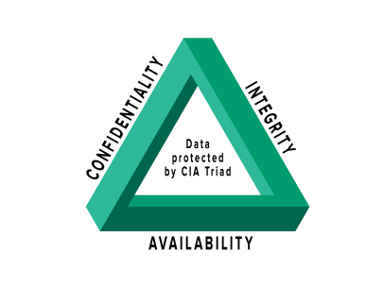
\includegraphics[width=0.5\textwidth]{CIATraid.png}
	\caption{Principes van het CIA Triad model (\cite{PrincipesCIA})}
	\label{fig:CIATraid}
\end{figure}

\subsection{Triple A }
Triple A of kortweg AAA, is de afkorting voor Authentication, Authorization en Accounting. Triple A definieert een architectuur die gebruikers authenticeert, autoriseert en de activiteiten logt. Met andere woorden wordt AAA gebruikt om de toegang te verschaffen naar elektronische systemen of netwerken.
\newline
\newline
Vaak spreekt men over een “open” netwerkarchitectuur wanneer AAA niet wordt toegepast binnen een infrastructuur. In deze “open” netwerkarchitectuur heeft iedereen toegang tot alle systemen, met als gevolg dat éénder wie alles kan uitvoeren zonder enige tracking.
\newline
\newline
In onderstaande alinea’s is er een zorgvuldige beschrijving van de drie A’s terug te vinden.
\subsubitem{\bf Authenticatie}
\newline
Tn dit proces wordt de identiteit van de persoon die een bepaalde dienst of service wenst te gebruiken nagegaan. Tijdens dit proces worden gegevens uitgewisseld om de identiteit van de gebruiker te kunnen verifiëren. Voorbeelden hiervan zijn: combinatie van gebruikersnaam en wachtwoord, het gebruik van een vingerprint scanning om in te loggen in bepaalde systemen, enz.
\newpage
\subsubitem{\bf Autorisatie}
\newline 
Autorisatie is het proces waarbij de rechten van iemand gecontroleerd wordt of hij beschikt over de juiste rechten om bepaalde diensten en/of services te contacteren. Met andere woorden wordt de vastgestelde identiteit gebruikt om te bepalen welke rechten de gebruiker heeft. Dikwijls wordt tijdens het vaststellen van deze rechten andere gegevens vastgelegd. Voorbeelden hiervan zijn: toewijziging van een IP adres, tijdslimiteringen, enz.

\subsubitem{\bf Accounting}
\newline
Accounting is het proces waarbij de gebruikte services of diensten van de vastgestelde gebruiker wordt bijgehouden. Deze informatie kan gebruikt worden voor doeleinden zoals management, facturatie, enz. Typische informatie die heel vaak wordt bijgehouden zijn, de vastgestelde identiteit van de gebruiker, het type dienst dat gebruikt werd of bepaalde tijdstippen wanneer men gebruik maakte van de verschillende diensten of services. 

\section{Bring Your Own Device}
BYOD staat voor “Bring Your Own Device”, ook wel "Bring Your Own Technology" genoemd. Dit is een concept waarbij iedereen binnen de organisatie zijn eigen apparatuur meebrengt naar het werk. Hierbij wordt veelal gerefereerd naar mobiele apparatuur, zoals smartphones, tablets, laptops, maar ook complete desktopcomputers die zakelijk gebruikt worden behoren ook tot deze trend. Deze talrijke systemen maken in vele situaties gebruik van de verschillende bedrijfsmiddelen zoals e-mail, file servers, databases en talrijke andere bedrijfsmiddelen.
\newline
\newline
De paper van \cite{Zakiah2017} meldt dat de opkomst van Bring Your Own Device behoorlijke opportuniteiten meebrengt voor hackers. Deze hackers vinden steeds meer nieuwe kwetsbaarheden die gevoelige data of informatie van werknemers of studenten uitbuit. Het zich bewust laten maken van deze veeltalige risico's aan de personen, is volgens \cite{Zakiah2017} de eerste stap tegen de opmars van online aanvallen op de 'Bring Your Own Technology' systemen.
\newline
\newline
Een uitgebreid beleid is dus een goede stap in de juiste richting om het bedrijfsnetwerk veiliger te maken, maar vaak is dit niet voldoende om het netwerk te bestendigen tegen cyberaanvallen. De implementatie van een network access control product kan hiervoor een oplossing bieden volgens \cite{Zakiah2017}.

\section{Internet of Things}
Als men aan Internet of Things (ofwel IoT) denkt, dan denkt men waarschijnlijk aan apparaten zoals smartphones of laptops, maar Internet of Things omvat veel meer dan dat. Het bestaat uit fysieke voorwerpen zoals huishoudelijke apparaten, wearables, kopieerapparaten, koelkasten of om het even welk fysiek apparaat dat met het internet verbonden is.
\newline
\newline 
Deze internetgebruikers worden de zogenaamde embedded systems genoemd. Zij kunnen communiceren met personen maar ook met andere embedded systems. Vaak is de communicatie simpel en eenvoudig, waardoor de embedded systems (ofwel Internet of Things apparaten) een kwetsbaarheid vormen in het bedrijfsnetwerk.
\newline
\newline
Wanneer er de paper van \cite{Salim2016} wordt bijgehaald, dan kan men afleiden dat Internet of Things infrastructuren en services, grote security uitdagingen ondervindt in elke omgeving. \cite{Salim2016} dicteerde het ‘Internet of Things security framework for smart infrastructures’ artikel die een duidelijker beeld schept over de integratie van smart homes of smart buildings met Internet of Things. Daarom ontworp \cite{Salim2016} een ‘threat model’ die een security methodologie voorstelt tegen cyber aanvallen. 
\newline
\newline
Om die reden is zoals bij Bring Your Own Device een uitgebreid beleid niet voldoende, maar kan een implementatie van een network access control product binnenin een bedrijfsomgeving de vruchten plukken op vlak van cybersecurity.  

\section{Network access control}
Nu reeds termen zoals Bring Your Own Device en Internet of Things uitgeklaard zijn, zal de betekenis en het belang van network access control technologieën verder uitgelegd worden.
\newline
\newline 
Een network access control is een type cyber security technologie waarmee ondernemingen beleidsregels kunnen implementeren en definiëren die de toegang van eind apparaten tot een bedrijfsnetwerk kunnen regelen. Tegelijkertijd biedt een network access control product een zichtbaarheid van apparaten die toegang proberen te krijgen met het netwerk, zodanig dat de veiligheid van het netwerk beter in kaart kan gebracht worden. Vervolgens wordt het belang van de implementatie van een network access control product in een netwerk toegelicht.
\newline
\newline 
Werknemers die met hun internet verbonden apparaten regelmatig inloggen op andere netwerken, maken de infrastructuur van hun eigen onderneming kwetsbaarder. Deze reizende systemen hebben een grotere kans om geïnfecteerd te worden met malware, dan apparatuur dat zich steeds binnen de muren van de onderneming bevindt. Een network access control product kan dus een oplossing bieden wanneer geïnfecteerde systemen toegang proberen te verschaffen in het netwerk. Dit is mogelijk dankzij Cisco's nieuwe 2.2 feature, namelijk Thread-centric access control. 
\newline
\newline 
De definitie en het belang van een network access control product werd alvast uitgelegd. In onderstaande alinea’s wordt er een woordje uitleg gegeven over drie nauwe, bijeenliggende network access control technologieën. Cisco Identity Services Engine werd gekozen in samenspraak met Axians. ‘Aruba ClearPass Policy Manager’ en ‘Portnox’ zijn network access control technologieën die willekeurig gekozen zijn op het internet. Vervolgens is er op het einde een kleine conclusie geschreven die dieper ingaat waarom er uiteindelijk gekozen werd voor Cisco Identity Services Engine en niet voor de overige network access control technologieën.

\subsection{Network access control technologieën}
\subsubsection{\bf Aruba ClearPass Policy Manager}
De Aruba ClearPass Policy Manager (\cite{ArubaCPPM})is een platform dat zorgt voor een veilige toegangscontrole tot een netwerk. Dit network access control (NAC) product is ontwikkeld omwille van de evolutie van smartphones, Bring Your Own Device en talrijke andere draadloze toepassingen. 
\newline
\newline
Netwerksecurity wordt de dag van vandaag steeds belangrijker en cyberaanvallen worden steeds geavanceerder. Met als gevolg moet privacygevoelige data binnen het netwerk blijven en mag enkel toegankelijk zijn voor geautoriseerde gebruikers. Aruba ClearPass Policy Manager biedt hiervoor een oplossing door gebruik te maken van een aantal uitgebreide zaken zoals o.a. , uitgebreide rapportages, ingebouwde AAA services zoals Radius, TACACS+, Kerberos, 802.1X, web radius authenticatie en dergelijke meer. In figuur \ref{fig:ArubaClearPass} zijn een aantal modules weergegeven binnen het Aruba ClearPass Policy Manager platform. 

\begin{figure}[H]
	\centering
	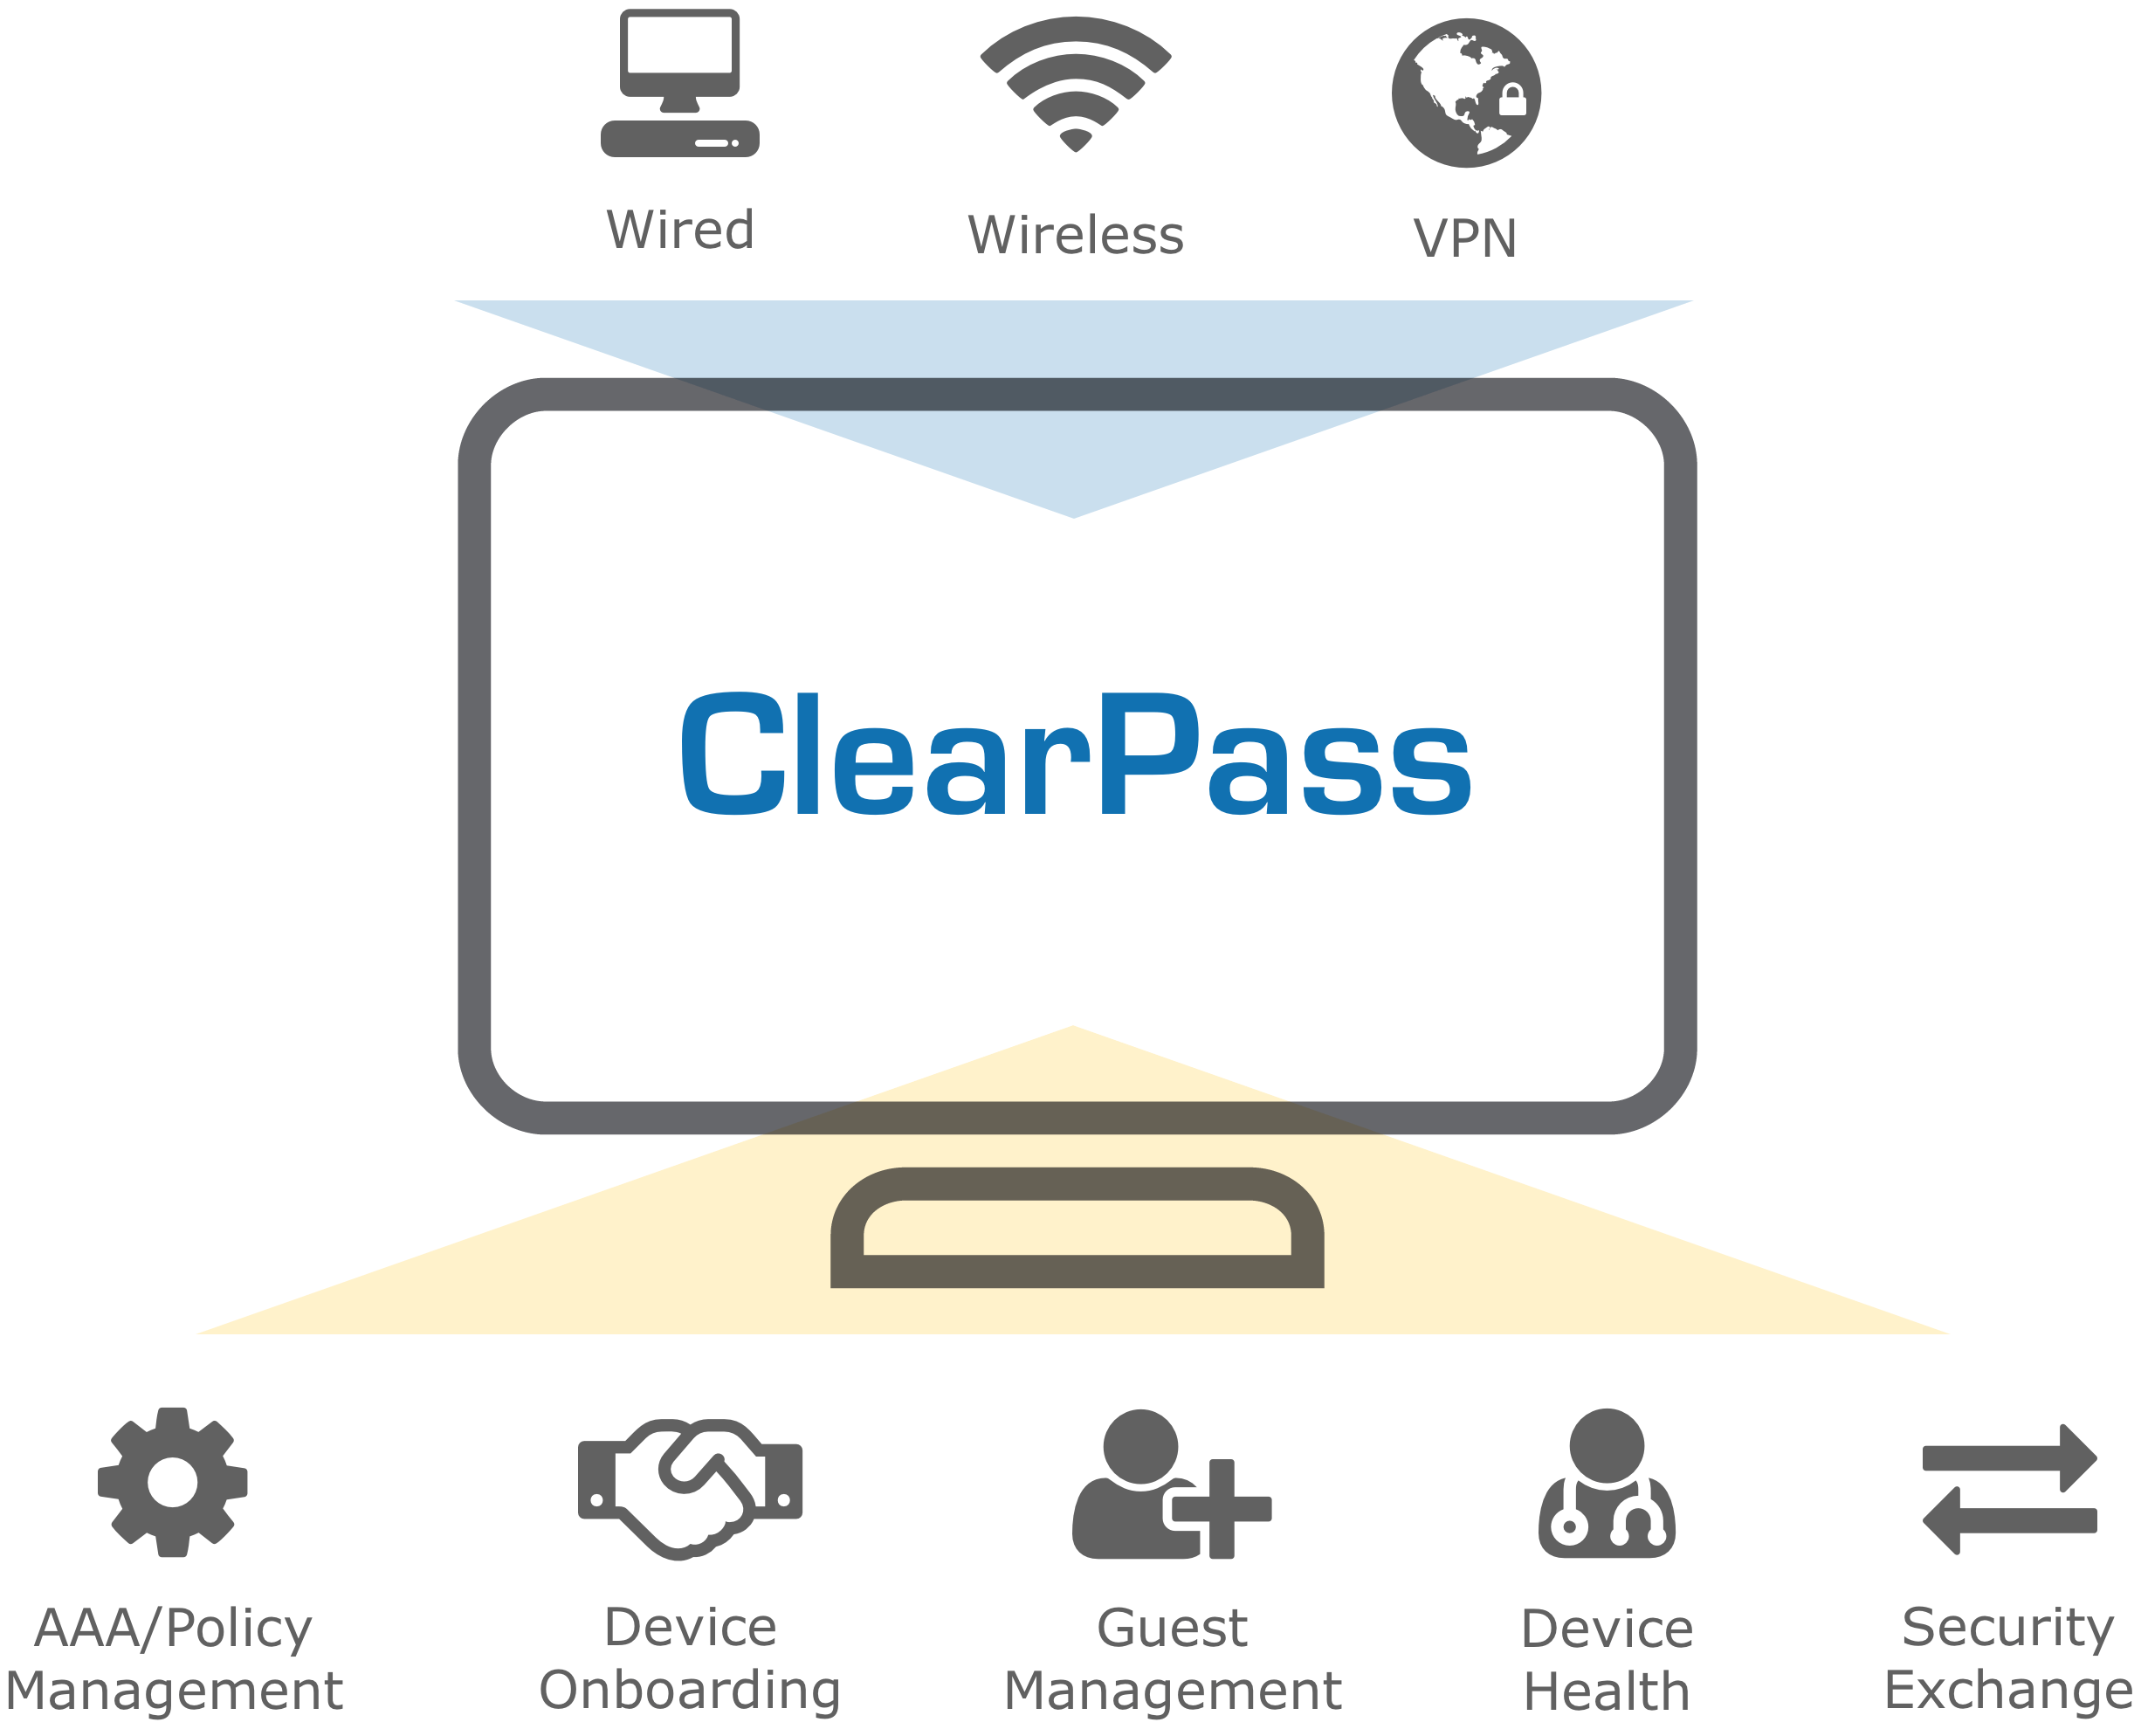
\includegraphics[width=0.5\textwidth]{Clearpass_authentication.png}
	\caption{Modules binnen het Aruba CPM platform (\cite{ACPMModule})}
	\label{fig:ArubaClearPass}
\end{figure}

\subsubsection{\bf Portnox}
Vervolgens is er het network access control technologie, genaamd \cite{Portnox}. Portnox is een network access control oplossing die vanuit de cloud wordt geleverd. Dit zijnde als ‘cloud as a service’. Desniettegenstaande dat dit ook mogelijk is om als on-premise gecentraliseerde software te gebruiken. Dit uit zich agentlesss op elk eind apparaat binnen in het bedrijfsterrein, of het nu Internet of Things is, Bring Your Own Device of door een ander bedrijf beheerd apparaat. In figuur \ref{fig:Portnox} is het logo van Portnox terug te vinden.
\newline
\newline
De veelzijdigheid van Portnox, maakt implementaties in de verschillende sectoren mogelijk. Dit zorgt er voor dat Portnox ook in het lijstje bevindt als competente kandidaten van network access control technologieën. Natuurlijk is het aanbod van competente network access control technologieën veel groter, maar deze literatuurstudie werd beperkt tot deze drie technologieën. 

\begin{figure}[H]
	\centering
	
\includegraphics[width=0.5\textwidth]{Portnox.png}
	\caption{Logo Portnox (\cite{PortnoxLogo})}
	\label{fig:Portnox}
\end{figure}

\subsubsection{\bf Cisco Identity Services Engine}
Cisco Identity Services Engine(\cite{ISE}) is een netwerkpunt waar alle methodes en identiteiten voor netwerktoegang worden geverifieerd aan de hand van gedefinieerde regelsets en authenticatiebronnen. Op basis van deze gedefinieerde regelsets en authenticatiebronnen kan Identity Service Engine toegangsrechten bieden tot bepaalde services. Factoren zoals: Active Directory groep, fysieke locatie van de gebruiker, OS-versie, enz. bepalen het type service dat gebruikt kan worden. Het doel is dus met andere woorden het vereenvoudigen van de identiteitsbeheer van de verschillende systemen en applicaties binnen het netwerk.
\newline
\newline   
Het radius protocol is één van de primaire communicatie protocol tussen Cisco Identity Services Engine en de verschillende eind apparaten binnen het netwerk.
\newline
\newline 
Remote authentication dial-in user service of Radius is een tripe A systeem, dat gebruikt wordt om de identiteit van een gebruiker die toegang wenst tot het netwerk vast te stellen. Met andere woorden zorgt Cisco Identity Services Engine voor een uitstekende zichtbaarheid van gebruikers en eind apparaten om mobiliteitservaringen van organisaties te ondersteunen en beter te beheren.
\newline
\newline
Door de unieke architectuur van Cisco Identity Services Engine kunnen bedrijven realtime data verzamelen van netwerken, gebruikers en eind apparaten. Vervolgens kan de beheerder deze informatie gebruiken om beleidsbeslissingen te maken door een identiteit te koppelen aan de verschillende netwerkelementen, waaronder draadloze LAN-controllers (WLC of Wireless Lan Controllers), virtual private network (VPN), datacenter switches, enz. 

\newpage
\subsubitem{\bf Policy-based access control}
\newline
Policy based access control(\cite{ABAC}), ook wel Attribute-based access control genoemd. Dit type access control definieert een toegang controleparadigma waarbij toegangsrechten worden verleend aan gebruikers door het gebruik van een beleid dat attributen combineert. Dit model ondersteunt de Booleaanse logica waarin beleidsregels "ALS en DAN" -instructies bevatten over wie het verzoek, de bron en de actie uitvoert.

\subsubitem{\bf Threat-Centric access control}
\newline
Het opstellen van de toegang controleparadigma op basis van de bedreiging- en kwetsbaarheid kernmerken is mogelijk via de Thread-Centric access control Identity Service Engine(\cite{TCNAC}) functie. Thread Centric access control ontvangt zijn bedreigingen- en kwetsbaarheid kernmerken op basis van één van de bedreigings- en kwetsbaarheids adapters. Het ernstniveau van deze bedreigingen en resultaten kan gebruikt worden om het toegangsniveau van een eind apparaat of eind gebruiker dynamisch te regelen.
\newline
\newline
Met andere woorden als een eind apparaat besmet zou raken met een virus, dan schiet de Threat-Centric access control functie in actie door dit eind apparaat in een vlan plaatsen die het netwerk niet verder kan infecteren. 

\subsubitem{\bf Port-based access control}
\newline
\cite{PBAC} definieert een client-server gebaseerde toegangscontrole en een authenticatieprotocol dat elke client verifieert voordat een service wordt aangeboden. Wanneer niet geautoriseerde apparaten verbinding wensten te maken met een openbare toegankelijke poort, dan laat de Port-based access control functie geen gewoon verkeer toe.
\newline
\newline
Tot deze client is geverifieerd, staat 802.1x-toegangscontrole alleen Extensible Authentication Protocol over het Local Area Network toe via de poort waarmee de client is verbonden. Wanneer de authenticatie geslaagd is, kan normaal verkeer de poort passeren.

\section{Voorgaande onderzoeken}
Een literatuurstudie zonder een degelijke en volwaardige verwijzing naar vorige onderzoeken, is natuurlijk geen volledige literatuurstudie. Daarom werd tijdens dit onderdeel van de literatuurstudie een aantal referenties gelegd naar vorige onderzoeken die een gelijkaardig studie hebben uitgevoerd.
\newline
\newline
De paper “Implementing NAP and NAC Security Technologies” van \cite{DanielV} meldt talrijke network access point en network access control oplossingen op real world hack scenarios. \cite{DanielV} presenteert dit aan de hand van talloze documentaties. Vervolgens is hoofdstuk 4 van het onderzoek: “Understation the need for LAN-based NAC/NAP” één van de belangrijkste hoofdstukken van de paper. Het artikel van \cite{DanielV} ligt aan de basis van dit onderzoek waarbij de implementatie van Cisco Identity Services Engine een oplossing biedt op een beter beheerbaar en veiliger bedrijfsnetwerk.
\newline
\newline 
Een recent onderzoek dat dateert uit 2018, geschreven door \cite{KevinDaimi}, laat lezers kennis maken met network access control producten die bedrijfsmiddelen beschermen tegen verschillende uitbuitingen. Deze paper behandelt een breed scala aan beveiligingsonderwerpen, waaronder netwerkbeveiliging, beveiligingsbeheer, informatieborging, beveiligingstoepassingen, computerbeveiliging, enz. Door concepten, technieken, methoden, benaderingen en trends te introduceren, kunnen organisaties hun beveiligingsvaardigheden en -capaciteiten verbeteren. 

\section{Literatuur conclusie}
Men kan pagina’s lang schrijven over bovenstaande network access control technologieën, maar men weet natuurlijk dat Cisco een groot voordeel heeft ten op zichte van andere network access control technologieën. Cisco is een wereldwijd erkend en zeer betrouwbaar product, die gekend is binnen de "Information Technology" wereld. De kwalitatieve verhoudingen van hun producten zijn zeker gekend, waardoor Cisco een groter publiek lokt in vergelijking met de rest.
\newline
\newline
Desniettemin zijn andere network access control technologieën zoals Portnox of Aruba ClearPass Policy Manager zeker waardige network access control producten. Zaken zoals het budget, de grootte van de onderneming of de kennis spelen vaak parten bij de selectie van een network access control. 
\newline
\newline
De keuze van het gebruik van Cisco Identity Services Engine heeft te maken omdat Axians gebruikt maakt van deze technologie. Vervolgens was de keuze van Cisco Identity Services Engine een meerwaarde voor beide partijen, hierdoor werd Cisco ISE gekozen. Verder worden er tijdens deze bachelorproef zeker en vast onderzoeken uitgevoerd waarom Axians koos voor Cisco Identity Services Engine en niet voor een network access control technologie zoals Aruba ClearPass Policy Manager of Portnox. Dit is mee verwerkt in de enquête.

